\documentclass[12pt]{article}
\usepackage[T1]{fontenc}
\usepackage{atbegshi}
\usepackage{graphicx}
\usepackage{hyperref}
\AtBeginDocument{\AtBeginShipoutNext{\AtBeginShipoutDiscard}}


\begin{document} \noindent
	\title{\Huge \textbf{Progetto Tecnologie Web}}
	\author{\textit{Preti Christian}}
	\date{2022}
	\maketitle 
	\noindent La relazione ha lo scopo di presentare il progetto svolto per il corso di \textit{Tecnologie Web}, ovvero un sito web per lo streaming di film e serie tv. \\ \\
	
	\noindent Saranno di seguito presentate le funzionalità principali del sito: \\
	\begin{itemize}
		\item Possibilità di recensire un film, con 1 $\sim$ 5 stelle e commento scritto.
		\item Panoramica delle recensioni scritte da un determinato utente.
		\item Lista di tutte le recensioni di un determinato film, con valutazione media.
		\item Ranking dei film in base alla valutazione media.
		\item Possibilità di cercare film in base al genere o con un voto minimo/massimo.
		\item Inserire un film tra i preferiti.
		\item Recommendation system operante sui generi preferiti di un utente, basandosi sulle recensioni di altri utenti a film guardati da entrambi.
		\item Chat di gruppo relativa ad un determinato film. \\
	\end{itemize}
	
	\noindent Nella prossima pagina verranno dati qualche approfondimenti su alcune di queste. 
	\pagebreak
	
	
	
	\noindent {\centerline {\Huge \textbf{Approfondimenti sui template}} \\ \par}
	
	\noindent \textbf{Home}: Essa contiene i form di login/registrazione. E' possibile anche accedere al sito come utenti anonimi, attraverso il tasto '\textit{Entra come guest}'. \\
	
	\noindent \textbf{Catalogo}: E' il catalogo del sito, al suo interno è possibile trovare la lista di tutti i film, con annessa \textbf{valutazione, generi, stato} (guardato/non guardato) e un \textbf{pulsante} che simula la possibilità di guardare il film. \\
	Cliccando sul titolo del film si verrà reindirizzati verso una pagina descrittiva più accurata, in cui sarà possibile avere informazioni aggiuntive quali, ad esempio, la trama. Inoltre, sempre nella pagina descrittiva del film, sarà possibile trovare un pulsante \textit{Chatta}, che appunto fornirà l'accesso, previa visione del film e login nel sito, alla chat di gruppo specifica del film. \\
	
	\noindent \textbf{Account}: Nella pagina \textit{Il mio account} sono presenti i vari \textit{componenti}:
	\begin{itemize}
		\item \textbf{Le mie recensioni}: Esso rappresenta un collegamento verso una pagina in cui sarà possibile avere una panoramica di tutte le recensioni lasciate dall'utente. Sarà inoltre possibile modificare i valori al suo interno, in caso l'utente avesse cambiato idea, oppure eliminarla completamente attraverso il pulsante dedicato.
		\item \textbf{Grafico}: E' un grafico di \textit{Chart.js}, è calcolato attraverso il metodo \textit{calcolaGeneri()}, presente nel file \textit{methods.py}.
		\item \textbf{Pulsanti blu}: Rappresentano un film \textit{guardato} dall'utente.
		\item \textbf{Pulsanti viola}: Rappresentano un film \textit{consigliato} dal \textit{recommendation system} all'utente.
	\end{itemize}
	
	\noindent \textbf{Ranking}: I parametri su cui è possibile fare ranking sono:
	\begin{itemize}
		\item \textbf{Titolo}.
		\item \textbf{Valutazione}, sia essa minima che massima.
		\item \textbf{Genere}. \\
	\end{itemize}
	
	\noindent \textbf{Chat}: Rappresentata come una semplice pagina in cui gli utenti, dopo aver necessariamente guardato il film, avranno modo di commentarlo con altri utenti.
	
	\pagebreak
	
	
	\noindent {\centerline {\Huge \textbf{Tecnologie utilizzate}} \\ \par}
	
	\noindent \textbf{Frontend}: Le tecnologie utilizzate lato frontend sono state: 
	\begin{itemize}
		\item \textbf{Bootstrap}: E' probabilmente il framework più utilizzato in ambito frontend, in grado di ricoprire i vari HTML, CSS e JavaScript. Ho fatto largo uso di Bootstrap, al fine di disegnare in modo facile e veloce le varie pagine del sito. \\
		
		\item \textbf{Chart.js}: E' una libreria che permette di importare grafici all'interno del proprio sito. È molto ben fatta, ben documentata e facile da usare. In questo contesto, è stata usata per disegnare un \textit{grafico poligonale} all'interno della pagina di account dell'utente. \\
		
		\item \textbf{AJAX}: Più che una tecnologia può essere vista come un'implementazione (o estensione) di JavaScript, che permette di creare richieste ad un server. E' molto importante perchè è uno strumento molto comodo quando si vuole interconnettere backend e frontend attraverso JavaScript, si pensi ad esempio al fornire al backend valori (più o meno complessi) ottenuti da elementi HTML quali tabelle o div. Facendo qualche esempio, in questo caso è stato utilizzato durante la fase di modifica ed eliminazione di una recensione, recuperando i valori dalla table attraverso JavaScript 'puro' e inviandoli con AJAX ad una Django view. \\ \\
	\end{itemize}

	\noindent Lato \textbf{Backend}, invece: 
	\begin{itemize}
		\item \textbf{SQLite}, data la comodità nel gestire il database in modo single-file e per la sua diretta integrazione con Django. \\
		
		\item \textbf{VSCode}, data la comodità nell'avere plugin che renderizzassero live le pagine HTML durante la scrittura, cosa che ha velocizzato molto il workflow. Inoltre, i plugin per la gestione dei test, facilmente avviabili in qualsiasi momento. Oltretutto, la possibilità di passare facilmente da un linguaggio di markup quale HTML o CSS, a Python/JavaScript. \\
		

		
		\item \textbf{Django}: E' il framework \textit{cuore} del progetto, dato che si occupa dell'interfacciamento con il database, della navigazione web, collegando ogni URL ad una view, della creazione dei modelli, creazione del superuser e del suo '\textit{admin panel}' (...) \\ \\
	\end{itemize}

	\noindent \textbf{Altri strumenti}:
	\begin{itemize}
		\item \textbf{SonarQube}: E' un software dedito all'ispezione di codice al fine di migliorarne la qualità. Permette anche di controllare il coverage, però essendo un po' complicato il link con Django, ho preferito gestire questo fattore attraverso il package 'Coverage.py', mentre ho usato SonarQube per tutti gli altri check sul codice, come il \textit{naming} delle variabili, lo \textit{smell code index}, quantità di \textit{bug} rilevati, il \textit{security hotspot index}...
		
		\item \textbf{Git/Github}: Per il \textit{version control} ho usato \textit{Git}, usando come servizio di hosting \textit{Github}. Fin dalle prime righe, il progetto è stato versionato sulla piattaforma.
	\end{itemize}
	\pagebreak

	
	\noindent {\centerline {\Huge \textbf{Divisione nelle varie app}} \\ \par} 
	Il progetto è stato diviso in 4 app:
	
	\begin{itemize}
		\item \textbf{Streamify}: È l'app principale del progetto, essa contiene tutti i templates e views, escluse quelle relative all'autenticazione e chat. In essa sono presenti \textbf{tutti} i model, ho preferito definirli tutti nella stessa applicazione in modo da aumentare l'ordine. \\
		
		\item \textbf{Chatify}: Come suggerisce il nome, essa fornisce il servizio di chat all'interno del sito. Ho deciso di separarla da Streamify, al fine di vederlo come un \textit{'servizio aggiuntivo'}, un po' come se fosse una feature esterna rispetto allo scopo \textit{principale} del progetto. \\
		
		\item \textbf{Auth}: Anche l'autenticazione è stata separata dal sito principale, dato che ho cercato di tenere le varie logiche quanto più separate possibili, al fine di aumentare la modularità del sito e la sua riusabilità. \\
		
		\item \textbf{Test\_Apps}: Essa contiene i test di tutte le app citate sopra, creando un'app dedicata a questo scopo mi è stato più facile gestirli, potendoli raggruppare tutti sotto la stessa directory. Ulteriori dettagli su questo verranno affrontati nel paragrafo dedicato. \\
	\end{itemize}
	\pagebreak
	
	\noindent {\centerline {\Huge \textbf{Ulteriori dettagli sulle funzionalità/scelte adottate}} \\ \par}
	
	\noindent \textbf{Recommendation System}: Esso è stato pensato come la somiglianza tra la doppia \{genere: voto medio\} di ogni utente verso ogni genere presente nel database.
	Inoltre, verranno dati suggerimenti solamente sui tre generi preferiti da utente, dato che difficilmente egli vorrà ricevere consigli su generi che non gli interessano. \\Questa lista di tre generi \textit{preferiti} verrà calcolata per ogni utente e verranno cercate delle corrispondenze tra gli elementi. Se trovati, si guarderà la differenza di voto medio al genere. Più la differenza sarà bassa, più si può presumere che i gusti, quantomeno su quel genere, tra i due utenti siano simili, e verranno consigliati all'utente loggato quelli guardati dall'altro utente, ma non da lui. \\
	Poniamo ad esempio:
	\begin{verbatim}
		U1: {
			'Azione': 4.5,
			'Avventura': 4.8,
			'Horror': 4,2
	}

	U2: {
		'Azione': 4.4,
		'Avventura': 5.0,
		'Fantascienza': 4,1
	}
	\end{verbatim}

	\noindent Ipotizzando che i tre generi preferiti dei due utenti siano quelli sopra citati, verrà trovato un match per i primi due generi, a questo punto bisogna calcolare la similarità, ovvero \textbf{quanto} il suggerimento può essere inerente, la formula sarà: \\
	
	$100 - {100 * |VotoGenereU1-VotoGenereU2| \over 5}$ \\ \\
	
	\noindent In questo esempio, all'utente U1 verranno suggeriti con una precisione del 98\% i film di genere \textit{Azione} guardati da U2 (ma ovviamente non da U1) e allo stesso modo con la precisione del 96\% i film di genere \textit{Avventura}. \\ \\
	
	\noindent \textbf{Gestione delle sessioni}: È stato fatto uso delle sessioni attraverso il dizionario associato a \textit{request}, ovvero \textit{request.session}. In esso sono stati salvati i valori che sarebbero stati utili durante tutta la durata della sessione attuale, al fine di poterli condividere con le varie views. \\
	Un esempio è il titolo del film che l'utente vorrebbe recensire, siccome la logica è stata '\textit{spezzata}' su due views, ho salvato il titolo del film nel dizionario di request in modo da poterlo condividere tra una view e l'altra. \\
	Le sessioni possono poi essere personalizzate in base alle proprie preferenze attraverso vari parametri, personalmente ho fatto uso dei seguenti, impostati nel file \textit{settings.py}:
	\begin{verbatim}
		SESSION_EXPIRE_AT_BROWSER_CLOSE = True
		SESSION_COOKIE_AGE = 240
	\end{verbatim}
	
	\noindent Con \textit{age} si intende la durata della validità, in secondi, della sessione, prima che il sito chieda di nuovo all'utente di effettuare l'accesso. \\ \\
	
	\noindent \textbf{Function-based views}: La mia scelta riguardo la scrittura delle views è ricaduta su quelle \textit{function-based}. Questo perchè fin da subito mi sono parse una scelta più \textit{ordinata} e \textit{intuitiva}. Soprattutto, in fase di scrittura mi sembrava di avere di più il controllo sulla logica vera e propria della view. \\ \\
	
	\noindent \textbf{Tipi di utenti}: Gli utenti, all'interno del sito, sono di 3 tipi:
	\begin{itemize}
		\item \textbf{Anonimo}: L'utente \textit{anonimo}, o anche \textit{AnonymousUser} è un utente coi permessi di base. Gli è concesso entrare nel catalogo attraverso il pulsante \textit{Entra come guest}, può solamente sfogliare il catalogo dei film e consultarne i dettagli, come titolo, valutazione media, anno di uscita...
		 
		\item \textbf{Loggato}: Un utente \textit{loggato} ha invece la possibilità di guardare un film, attraverso un pulsante presente in corrispondenza del film, nel catalogo. Ha la possibilità di consultare la propria pagina \textit{Il mio account}, per avere la lista dei film da egli guardati, le recensioni lasciate e i film suggeriti dal recommendation system. Sempre in questa pagina è presente anche il grafico reso disponibile da Chart.js, che mostra in modo user-friendly i generi preferiti.
		\item \textbf{Admin}: L'utente \textit{admin} è inteso come l'amministratore/gestore del sito. Ha il permesso di aggiungere, modificare ed eliminare utenti, film e generi. \\
	\end{itemize}

	\noindent La gestione degli utenti è stata ripresa da quella \textit{base} di Django, ovvero il modello \textit{Utente} altro non è che un'estensione della classe \textit{AbstractBaseUser}, fornito direttamente da Django. \\
	Le classi da cui un custom user può essere esteso sono AbstractBaseUser e AbstractUser, nel mio caso ho scelto la prima, dato che si tratta di una versione quanto più \textit{basic} possibile, al fine di poterla personalizzare a mio piacimento. \\
	Se si fa uso di AbstractUser/AbstractBaseUser, bisogna specificare a Django quale modello verrà interpretato come utente, ciò è possibile inserendo nel file \textit{settings.py} la seguente riga: \\ \\
	AUTH\_USER\_MODEL = 'streamify.Utente' \\ \\
	Estendere un utente da AbstractBaseUser porta notevoli benefit rispetto a crearlo \textit{from-scratch}, dato che fornisce la possibilità di usare vari decoratori (anch'essi già forniti da Django) e metodi per il controllo sugli utenti. Ad esempio: 
	
	\begin{itemize}
		\item \textbf{login\_required}: Come ci suggerisce il nome, viene usato per decorare una funzione che necessita di un utente effettivamente loggato per essere eseguita.
		
		\item \textbf{authenticate}: Altro non è che una funzione che prende in input un set di credenziali (solitamente username/email e password), fa un check nel database cercando nel modello definito come utente e, in caso di match, ritorna l'oggetto desiderato.
		
		\item \textbf{login}: Una volta aver ottenuto un utente attraverso authenticate() e quindi essersi accertati che, dato il set di credenziali, esista effettivamente un tale utente nel database, sarà possibile \textit{assegnarlo} alla sessione corrente, attraverso appunto questa funzione. \\ \\
	\end{itemize}
	
	\noindent \textbf{Status codes}: Gli status codes sono una parte fondamentale nello sviluppo di un applicativo web, dato che forniscono il modo per diversificare l'esito delle varie operazioni. Essi sono stati utili durante la scrittura dei test, dato che mi è stato possibile usarli per confermare che l'esito di una determinata operazione fosse quello atteso. Possono essere inseriti manualmente e passati come parametro durante il return del render di una view, con parametro \textit{status}. \\ \\
	
	\noindent \textbf{Template tags}: Un template tag è una sorta di funzione applicabile ad un template. Nel mio caso ne ho implementata solamente una, chiamata \textit{replace\_titles}, la sua funzione è quella di prendere in input il titolo di un film, che avrà dei \_ al posto dei whitespace (per comodità nei link, quando passato come parametro GET), e sostituirà quest'ultimi con dei whitespace appropriati, si tratta quindi solamente di un workaround \textit{grafico}. \\ \\
	
	\pagebreak
	\noindent {\centerline {\Huge \textbf{Modelli}} \\ \par}
	
	\noindent All'interno del progetto sono presenti 4 entità:
	
	\begin{itemize}
		\item \textbf{Utente}: Il modello Utente eredita dalla classe padre \textit{built-in} di Django, \textbf{AbstractBaseUser}. La particolarità di quest'ultima, rispetto a \textbf{AbstractUser}, è l'essere il più minimale possibile, esso infatti è composto solamente di \textit{password} e \textit{last\_login}.\\ \\
		Un utente è stato definito dai seguenti \textit{fields}:
		\begin{itemize}
			\item \textbf{username}
			\item \textbf{email}
			\item \textbf{password}
			\item \textbf{nome}
			\item \textbf{cognome}
			\item \textbf{is\_active} --> Alternativa all'eliminazione dal DB di un utente in situazioni come un \textit{blocco temporaneo} dell'account.
			\item \textbf{is\_staff} --> Booleano che indica se un utente può accedere alla pagina di admin.
			\item \textbf{is\_superuser} --> Booleano che indica se un utente ha i permessi di admin.
			\item \textbf{date\_joined} --> Data in cui l'utente si è registrato al sito.
			\item \textbf{last\_login} --> Data in cui l'utente ha effettuato l'accesso l'ultima volta.
		\end{itemize}
		
		\item \textbf{Film}:
		\begin{itemize}
			\item \textbf{titolo}
			\item \textbf{generi}
			\item \textbf{anno\_uscita}
			\item \textbf{trama} \\
		\end{itemize}
		
		
		\item \textbf{Genere}:
		\begin{itemize}
			\item \textbf{name}: Rappresenta il nome del genere, e.g. \textit{Azione, Avventura...} \\
		\end{itemize}
		
		
		
		\item \textbf{Recensione}:
		\begin{itemize}
			\item \textbf{voto}: Rappresenta il voto numerico della recensione, con range 1$\sim$5.
			\item \textbf{film}: \textit{Foreign Key} di \textit{Film} che specifica il film recensito.
			\item \textbf{utente}: \textit{Foreign Key} \textit{Utente} che specifica l'utente autore della recensione.
			\item \textbf{commento\_scritto}: Commento scritto opzionale.
		\end{itemize}
	\end{itemize}

	\noindent E' presente poi lo UserManager, ovvero un'estensione della classe padre BaseUserManager, il cui scopo è quello di gestire la creazione di nuovi utenti. Esso verrà chiamato durante la creazione di un utente attraverso la seguente operazione, presente nel modello Utente:\\ \noindent objects = UserManager() \\ \\
	Lo UserManager creerà attraverso il metodo \textit{\_create\_user(self, email, password, **extra\_field)}, l'utente. \\
	Da notare bene, lo UserManager si occupa della creazioni di utenti che possono sia essere utenti normali del sito, ma anche amministratori. La diversificazione nella creazione dei due avviene attraverso due metodi separati:
		\begin{itemize}
			\item Con il comando 'python manage.py createsuperuser' verrà chiamato il metodo di UserManager create\_superuser, che a sua volta chiamerà il metodo \_create\_user() con is\_staff e is\_superuser settati a 'True'.
			\item Attraverso il form di registrazione presente nella home del sito, verrà creato un utente \textit{normale} e verrà chiamato il metodo create\_user di UserManager, che invece  chiamerà il metodo \_create\_user() con is\_staff e is\_superuser settati a 'False'.
		\end{itemize}
	
	\noindent Inoltre, lo UserManager setterà la password con il metodo \textit{set\_password()}, che effettuerà l'hash della password per aumentarne la sicurezza.

	\pagebreak
	
	
	\noindent {\centerline {\Huge \textbf{Testing}} \\ \par}
	
	\noindent Come specificato nel paragrafo riguardo alla divisione in più app, i test sono stati separati dal resto delle applicazioni, questo ha permesso di facilitare la loro gestione, permettendomi di raggrupparli tutti sotto la stessa app. Dentro il path ./test\_apps/tests/, possiamo trovare varie directory. \\Ho deciso di separare anche qui i test al fine di tenerli ordinati e poter, su richiesta, eseguire test riguardanti un preciso/alcuni argomenti. \\
	Per i test mi sono affidato a \textit{Django Unit Test Framework}, che sfrutta nativamente \textit{unittest}.
	Sono presenti più test per ogni singola view, dato che è stato testato ogni possibile aspetto di ogni view, ovvero il caso di \textit{success}, \textit{fail} e \textit{conflict}. \\ \\
	Per orientarmi durante la scrittura di un test, è stato utile assegnare lo status code manualmente ad ogni render delle view, alcuni esempi:
	\begin{itemize}
		\item Se l'utente effettua l'accesso con successo, lo status code sarà 200 (\textbf{Successo}).
		\item Se l'utente inserisce credenziali errate, lo status code sarà 401 (\textbf{Unauthorized}).
		\item Se l'utente si registra con username o email già in uso, lo status code sarà 409 (\textbf{Conflitto}).
	\end{itemize}

	\noindent I test verranno \textit{eseguiti} da \textbf{coverage.py} un package fornito da PIP, con cui Django si è dimostrato veramente ben integrato. Coverage può cercare, attraverso il parametro '--source' all'interno di path specifici, motivo per cui ho tenuto a separare i vari tipi di test. Di seguito, verrà riportato un resoconto del coverage dell'intero progetto:
	
	\begin{center}
		\centering 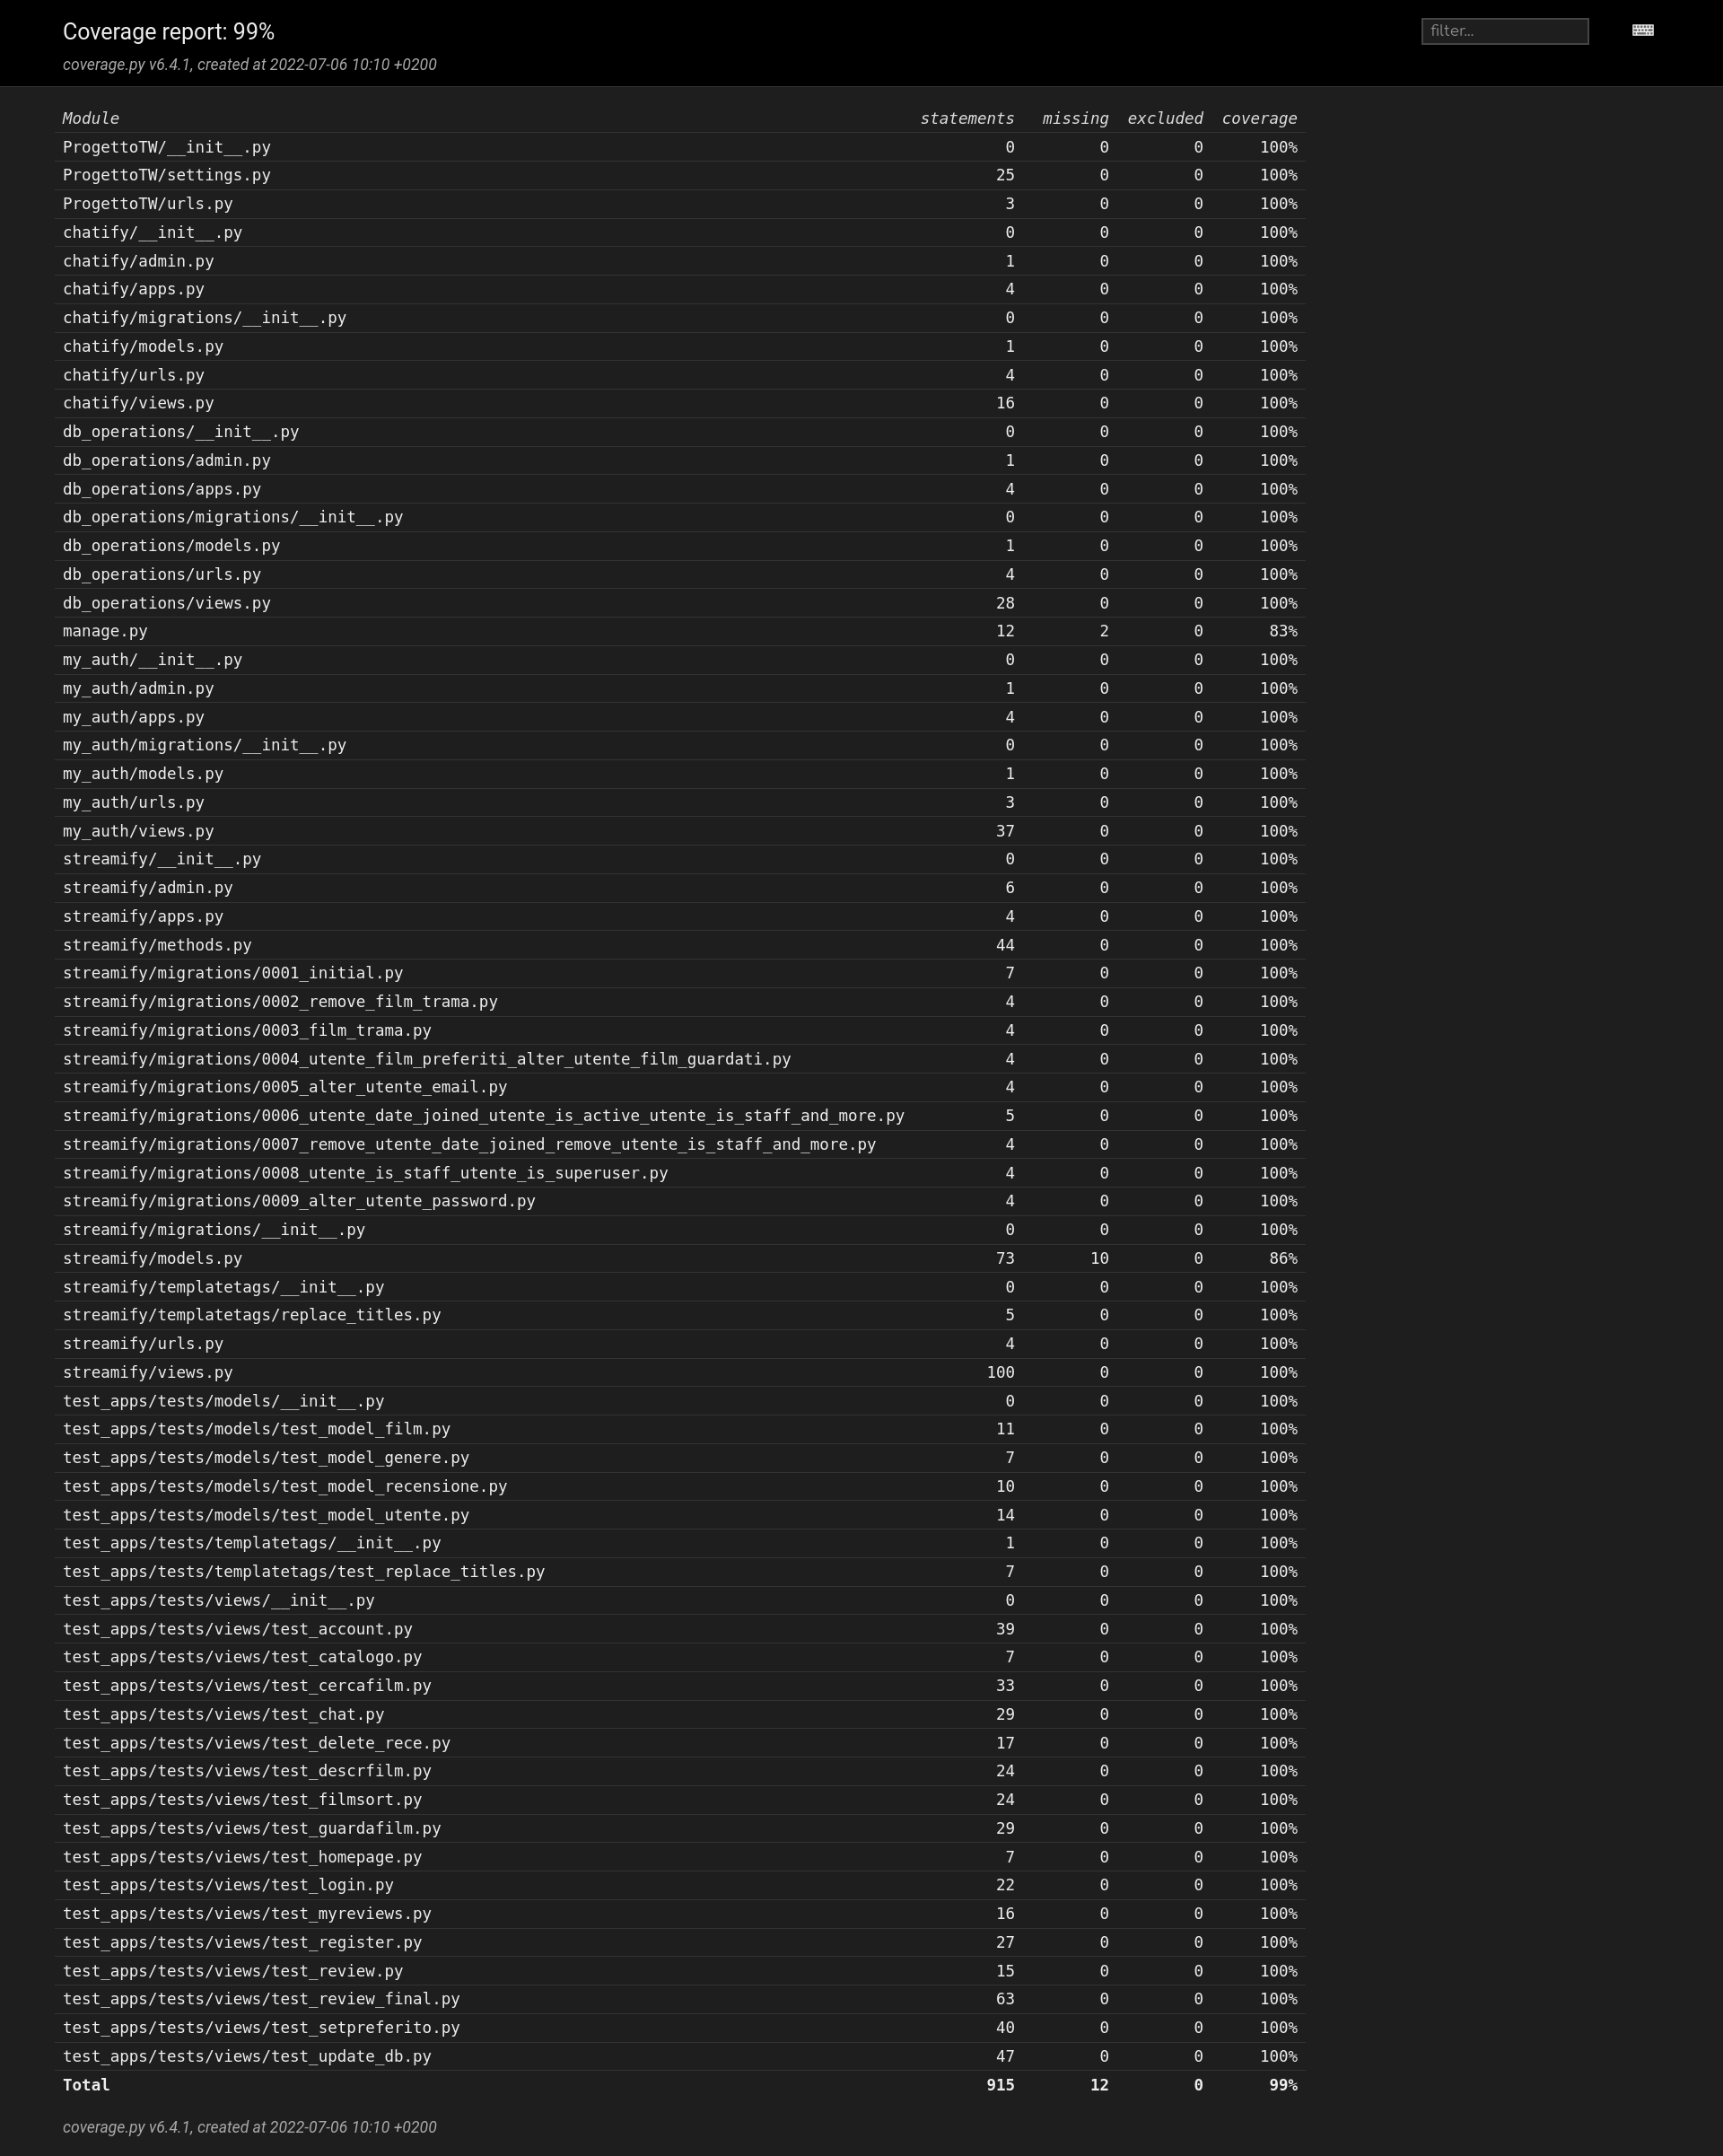
\includegraphics[width=11cm]{Immagini/coverage_report.png} \\
		\centering Coverage report	
	\end{center}
	\pagebreak
	
	
	\begin{center}
		\noindent {\centerline {\Huge \textbf{Schemi}} \\ \par}
		\centering 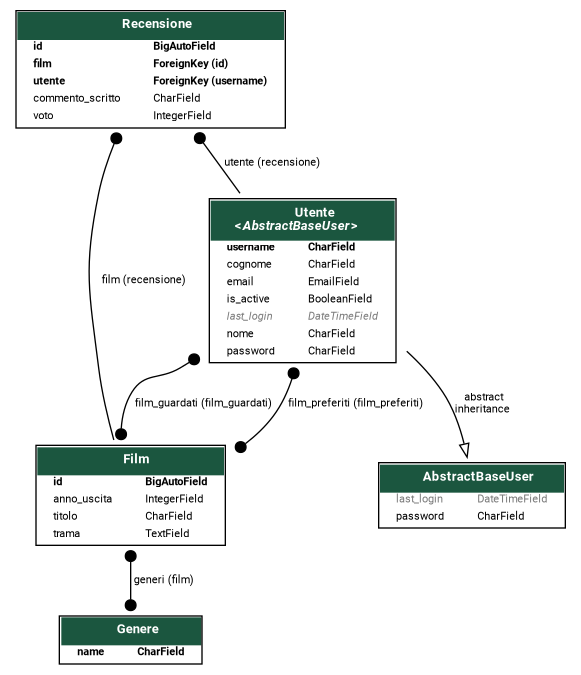
\includegraphics[width=11cm]{Immagini/streamify.png} \\
		\centering UML Schema
	\end{center}
		\pagebreak
		

	\begin{center}
		\noindent {\centerline {\Huge \textbf{Screenshot più interessanti}} \\ \par}
		\centering 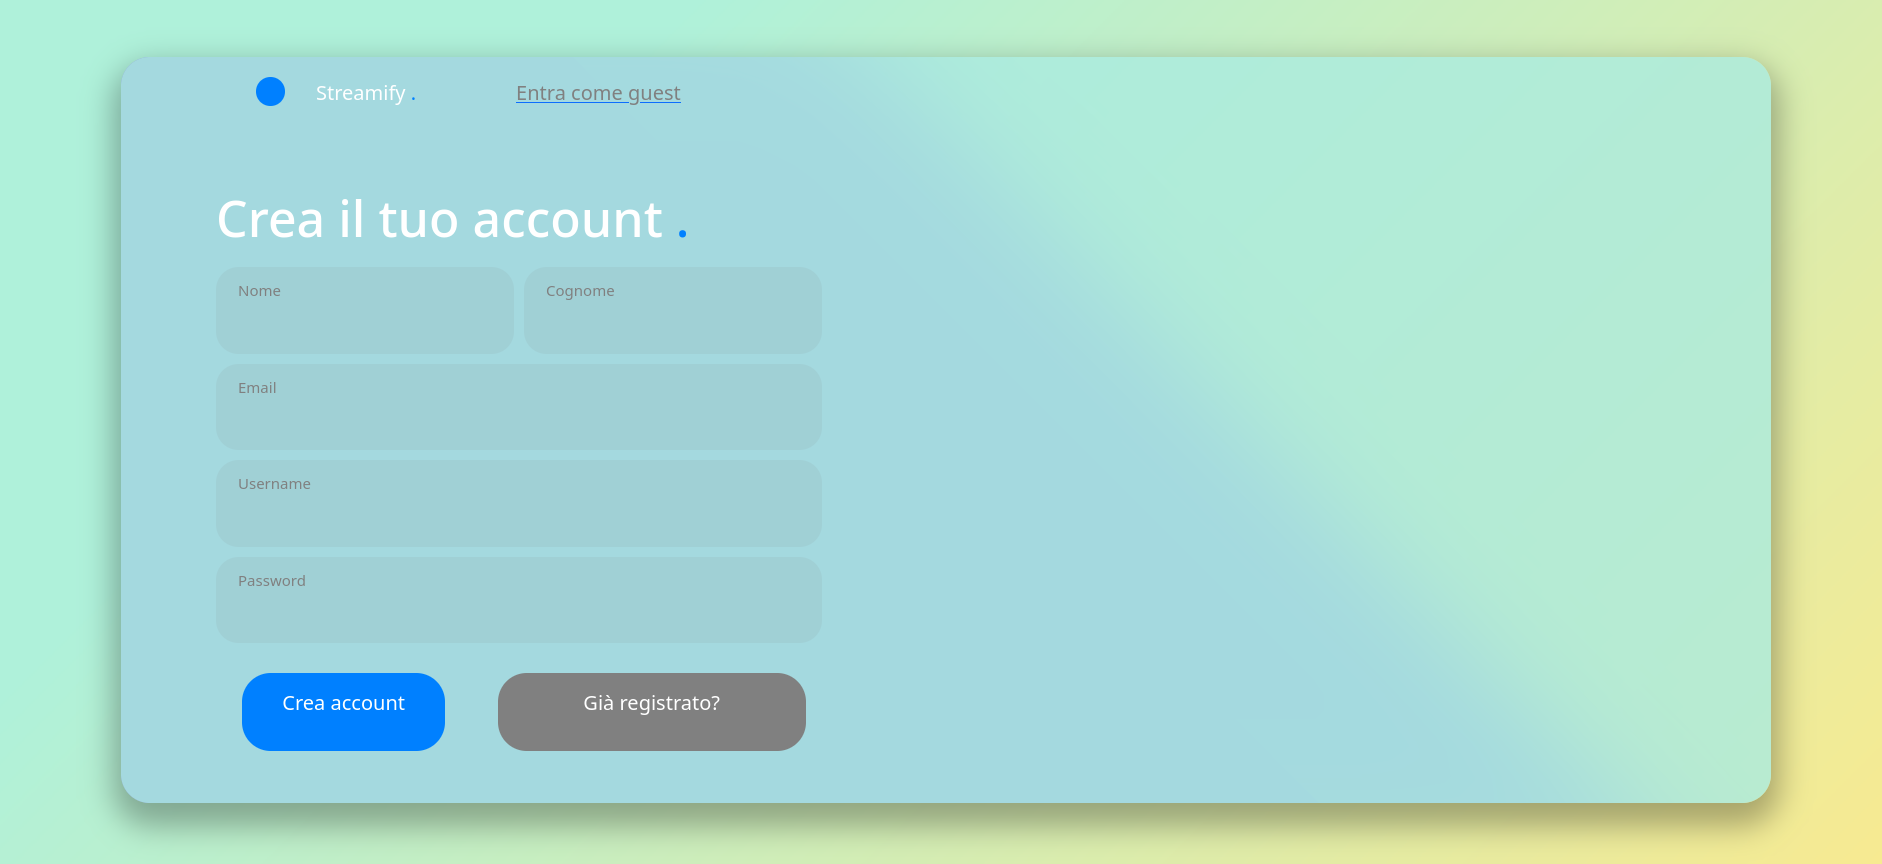
\includegraphics[width=15cm, height=7cm]{Immagini/Home_screen.png} \\
		\centering Screenshot della home ~\\ ~\\ ~\\ ~\\ ~\\
		
		\centering 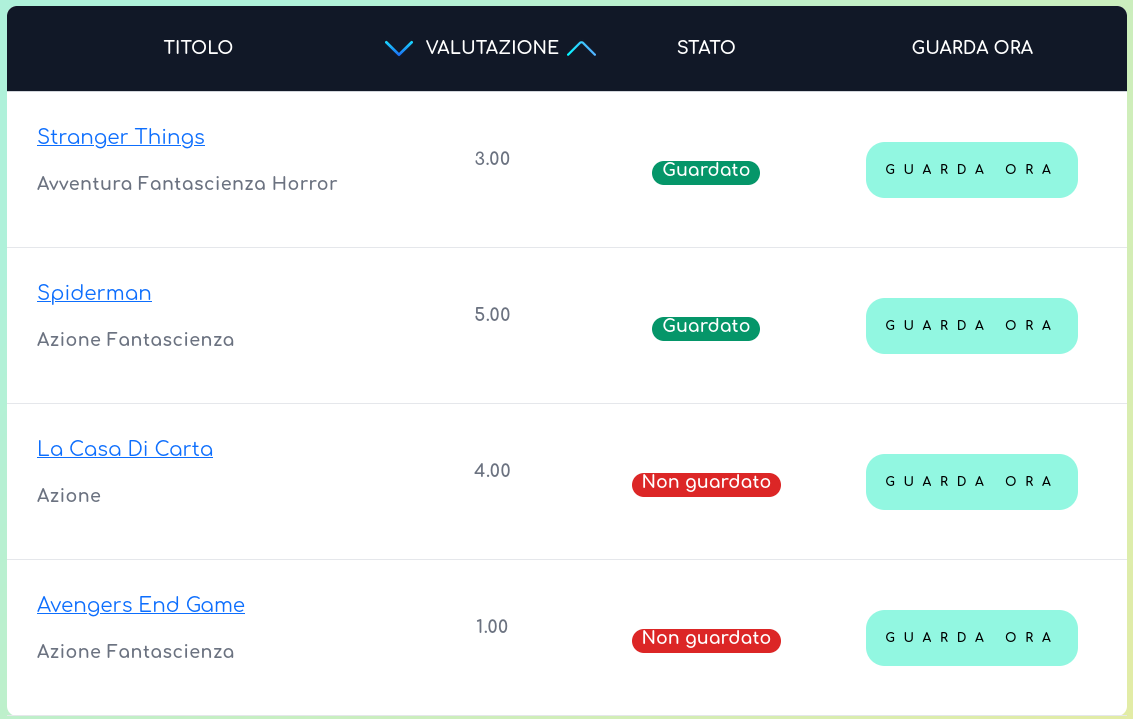
\includegraphics[width=15cm, height=8cm]{Immagini/Catalogo_screen.png} \\
		\centering Screenshot del catalogo
		
		\centering 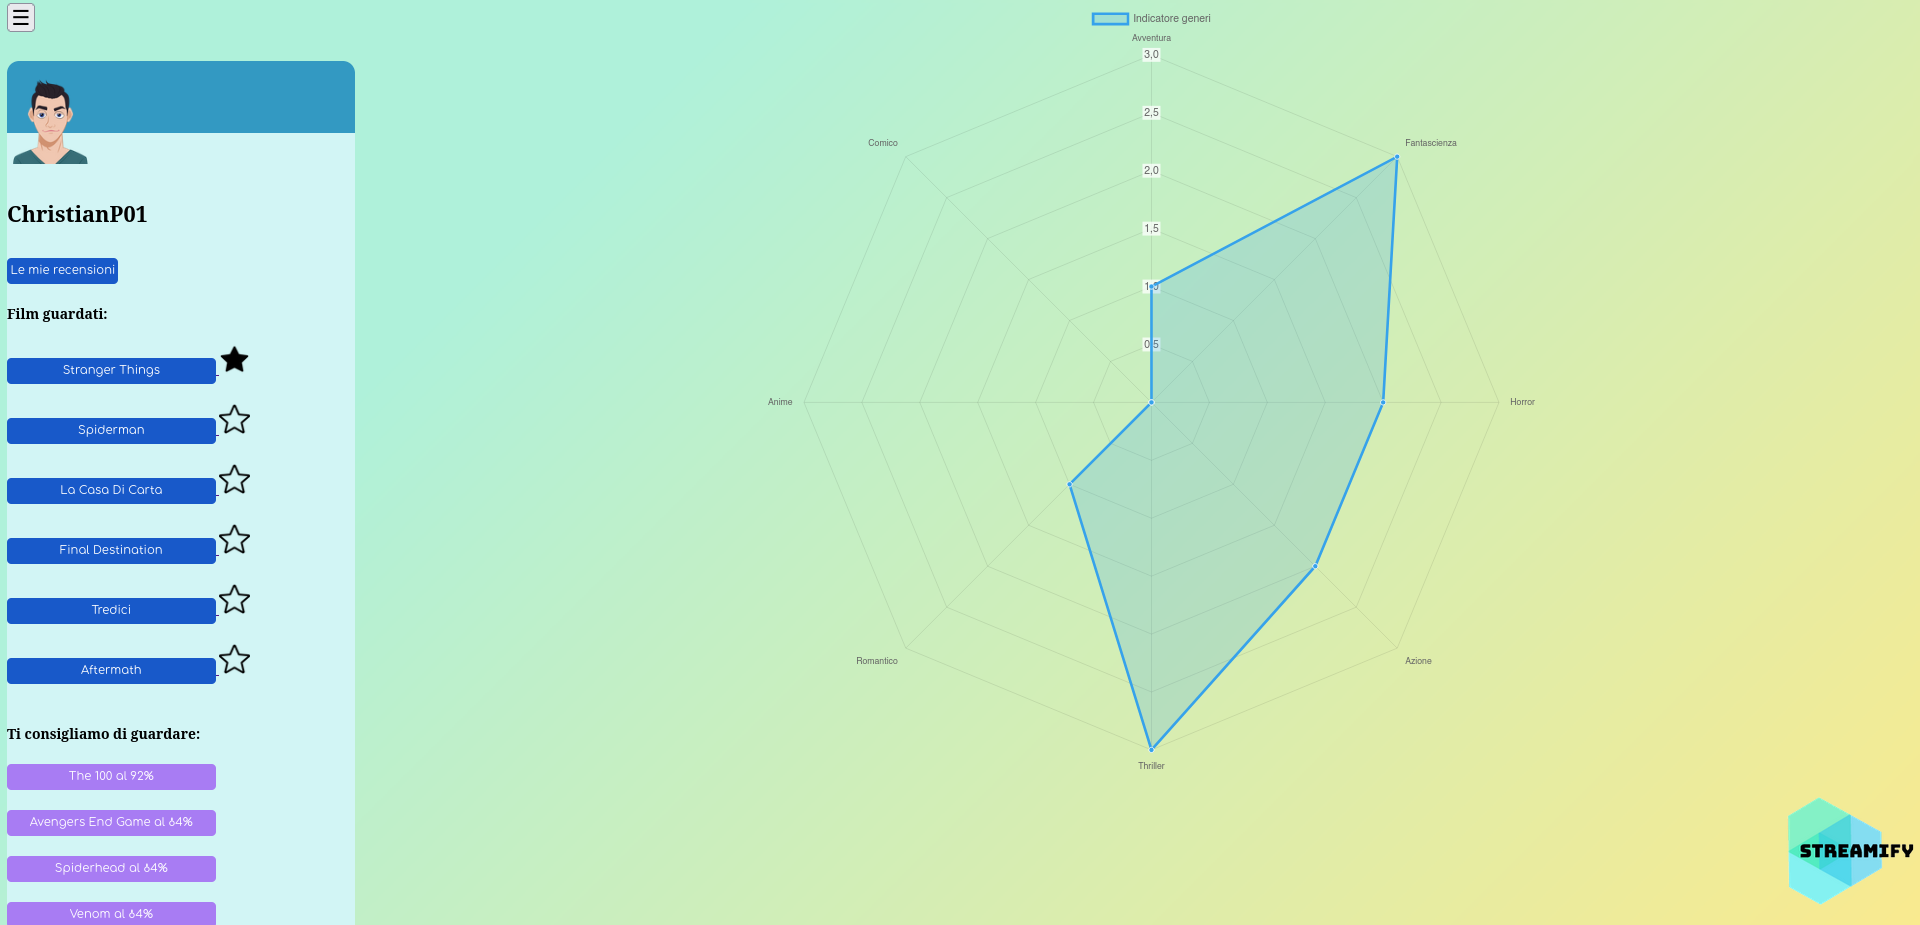
\includegraphics[width=15cm, height=7cm]{Immagini/Account_screen.png} \\
		\centering Screenshot dell'account page ~\\ ~\\ ~\\ ~\\ ~\\
		
		\centering 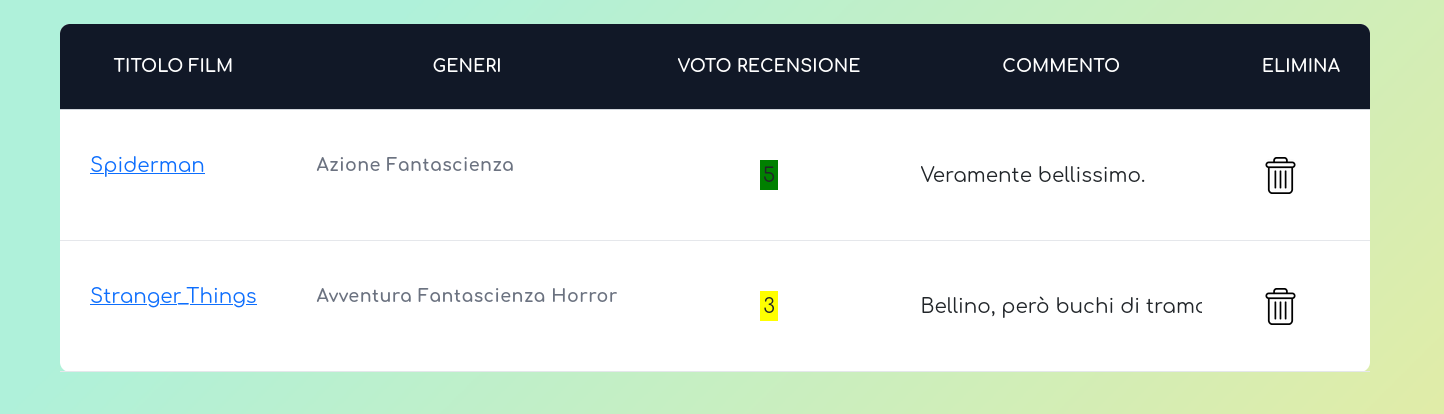
\includegraphics[width=15cm, height=6cm]{Immagini/User_reviews_screen.png} \\
		\centering Screenshot delle recensioni scritte dall'utente
	\end{center}
	\pagebreak
	
	
	\noindent {\centerline {\Huge \textbf{Problemi riscontrati e commenti finali}} \\ \par}
	
	\noindent Di problemi in sè non ne ho trovati particolarmente, o comunque nulla che tramite qualche ricerca su Internet non possa essere risolto. D'altronde è il framework più utilizzato nel suo ambito, e la documentazione che è possibile trovare nei vari forum è elevatissima. \\
	Ci sono alcune cose che non mi hanno del tutto convinto, durante lo sviluppo del progetto. \\
	Ad esempio, Django tratta i QuerySet come liste di oggetti che matchano un filtro (query), sarebbe stato più comodo dare la possibilità di modificarli attraverso qualche metodo. Nel mio caso, nel recommendation system, se avessi avuto la possibilità di intervenire sugli elementi di un QuerySet (ad esempio potendo aggiungere o eliminare elementi), avrei potuto evitare di instanziare oggetti 'pressochè inutili'. Questo da un certo punto di vista ha senso, perchè si tratta comunque di una query e sarebbe concettualmente sbagliato intervenirci manualmente, anche se in alcune situazioni, appunto, sarebbe stato comodo. Apparte questo dettaglio, gli altri problemi riscontrati sono stati minori e risolvibili con qualche ricerca online. \\ \\
	Per concludere, devo dire che come corso mi è piaciuto fin da subito, soprattutto considerando la modalità d'esame. Credo infatti si possa imparare \textit{molto} di più dallo sviluppo di un progetto, soprattutto su un argomento del genere. È stata la mia prima esperienza riguardo lo sviluppo web e ne sono rimasto soddisfatto. Mi ha insegnato molto sia dal punto di vista strutturale di un progetto (divisione in app, ordine nella struttura delle directory, test) e di come frontend e backend effettivamente riescano a comunicare. \\
	
	
	
	

\end{document}